\section{Methodology}
\label{sec:methodology}

Motivated by the compute and latency constraints of edge devices \cite{9, 20, 21}, and the observation that compact models relying on parallel dilated convolutions can exhibit sensitivity to input scale variations \cite{5, 16}, this work introduces Multi-Scale Consistency Gated Test-Time Augmentation (MCG-TTA). The underlying hypothesis is that scale-induced ambiguity in compact multi-dilation architectures concentrates in low-confidence predictions, and that these predictions can be stabilized at inference time by probing the model with multi-scale views aligned with its internal dilation structure, requiring no additional learned parameters.

In this section, we formulate the image classification problem, analyze the spatial scale sensitivity of compact atrous convolutions, present the algorithmic stages of MCG-TTA, derive an analytical latency model, and define the patient-level volumetric diagnostic aggregation.

\subsection{Problem Formulation and Base Network Architecture}

Let $\mathbf{I} \in \mathbb{R}^{H \times W \times C}$ denote a 2D brain MRI slice, where $H, W$ represent spatial dimensions and $C$ denotes channel dimensionality. A deep neural network $f_\theta$ parameterized by learned weights $\theta$ maps the input slice to a vector of logits $\mathbf{z} = f_\theta(\mathbf{I}) \in \mathbb{R}^K$ over $K$ mutually exclusive diagnostic categories. 

The predicted class posterior probabilities are computed via the softmax operator:
\begin{equation}
\mathbf{p} = \sigma\left(f_\theta(\mathbf{I})\right) \in \Delta^{K-1}, \quad \text{where } p_c = \frac{\exp(z_c)}{\sum_{j=1}^K \exp(z_j)}
\label{eq:softmax}
\end{equation}
The model's predictive confidence is quantified by the maximum posterior probability:
\begin{equation}
p_{\max} = \max_{c \in \{1, \dots, K\}} p_c
\end{equation}
with initial predicted class $c_0 = \arg\max_c p_c$.

To support execution on resource-constrained hardware, we adopt a compact multi-scale convolutional architecture as the base backbone (specifically LiteSpeed-Net \cite{16}). As illustrated in Fig.~\ref{fig:lsnet-architecture}, the backbone incorporates multi-path atrous (dilated) depthwise convolutions (MPAC blocks \cite{16}) to expand the effective receptive field without parameter inflation, allowing the network to capture both local tissue textures and broader anatomical context.

\begin{figure*}[t]
\centering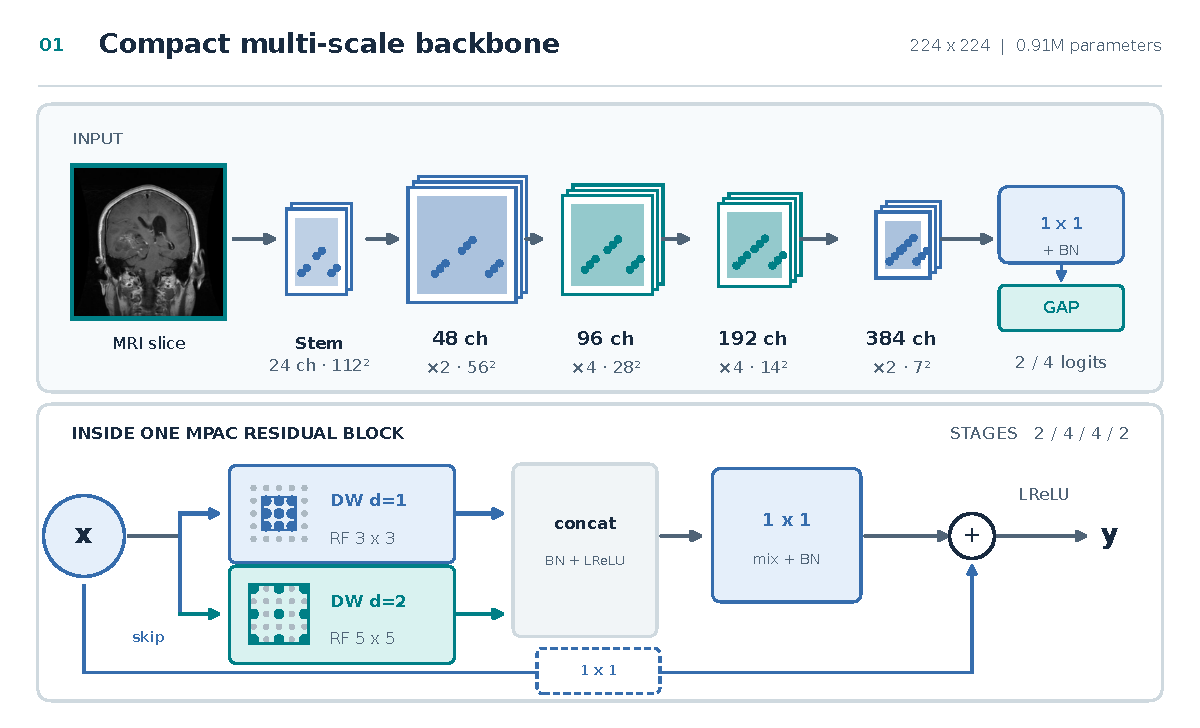
\includegraphics[width=0.88\textwidth]{figures/lsnet_architecture.pdf}
\caption{Architecture of the compact LiteSpeed-Net (LS-Net) backbone and MPAC residual block.}\label{fig:lsnet-architecture}
\end{figure*}

\subsection{Spatial Scale Sensitivity in Compact Atrous Convolutions}

While atrous convolutions expand the receptive field without downsampling spatial resolution \cite{5}, their discrete sampling mechanics introduce structural sensitivity under input distribution shifts.

An atrous convolution with dilation rate $d > 1$ samples input features on a sparse regular lattice with stride $d$. In deep, overparameterized architectures, the resulting sparse sampling artifacts, commonly termed the \emph{gridding effect} \cite{5}, are mitigated by dozens of subsequent parameterized layers that continuously blend feature maps across deep residual stages. In contrast, compact vision models designed for low-power edge environments \cite{16} possess limited parameter depth, restricting their capacity to interpolate across discrete spatial sampling gaps.

When deployed across clinical environments with differing acquisition settings (such as variations in slice thickness, scanner geometry, or lesion dimensions), pathological margins undergo spatial scale shifts relative to the training distribution. Consequently, fixed dilated sampling points can misalign with fine anatomical boundaries, such as thin infiltrative borders or micro-structural margins \cite{5, 16}.

Based on these observations, we formulate two design principles:
\begin{enumerate}
\item \emph{Uncertainty Concentration}: Spatial scale sensitivity manifests primarily in predictions exhibiting high predictive uncertainty ($p_{\max} < \tau$, where $\tau$ denotes an empirical confidence threshold).
\item \emph{Architecture-Informed Scale Probing}: Because this sensitivity stems from discrete spatial sampling intervals, uncertain predictions can be probed and stabilized at test time by applying targeted scale perturbations that mirror the internal dilation offsets of the architecture, without altering the model's learned parameters.
\end{enumerate}

\subsection{Multi-Scale Consistency Gated Test-Time Augmentation (MCG-TTA)}

To improve inference robustness while strictly bounding computational overhead, we formulate Multi-Scale Consistency Gated Test-Time Augmentation (MCG-TTA). Instead of applying test-time augmentation unconditionally across all inputs, which scales inference latency linearly with the number of views \cite{42}, MCG-TTA dynamically routes samples through a three-stage decision pipeline, as depicted in Fig.~\ref{fig:mcg-tta}.

\begin{figure*}[t]
\centering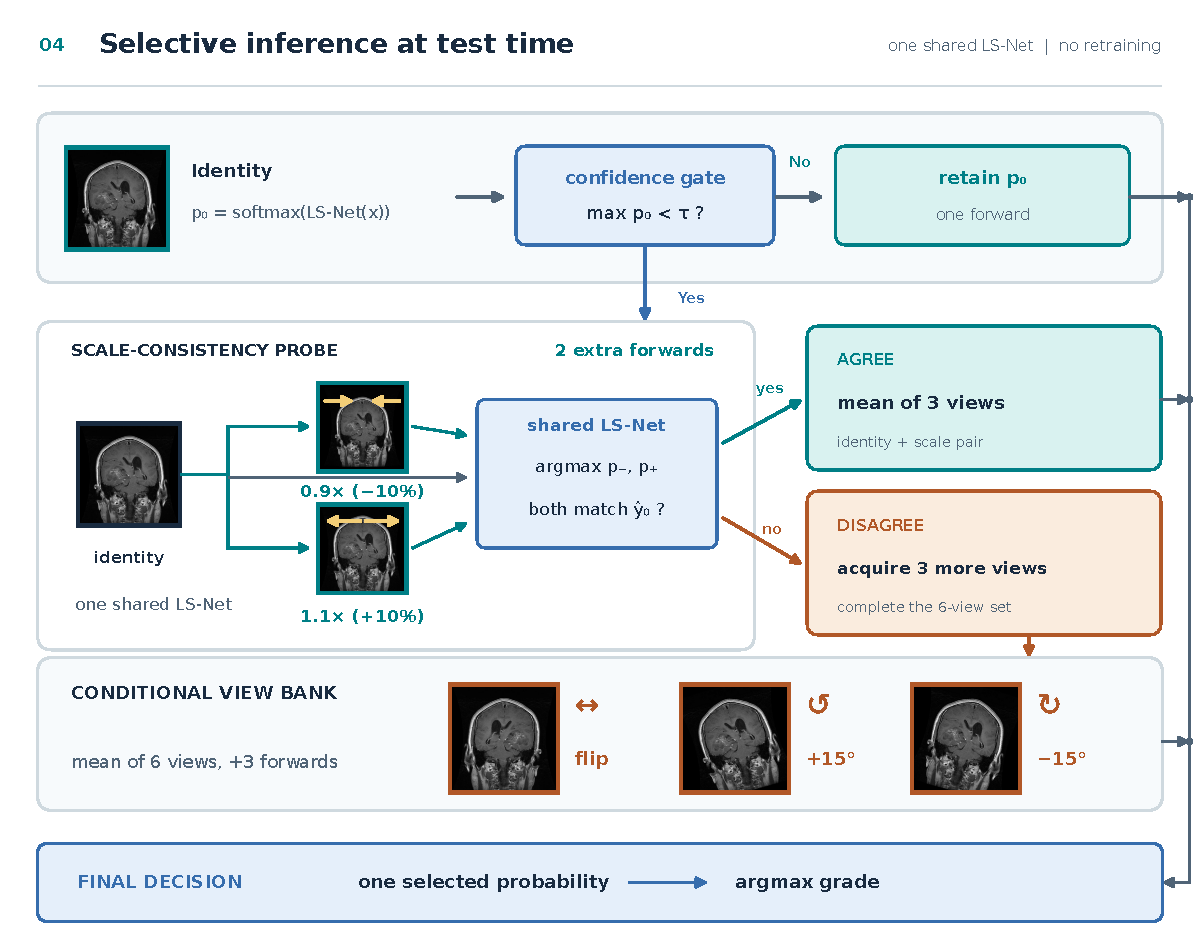
\includegraphics[width=0.85\textwidth]{figures/mcg_tta.pdf}
\caption{Decision pipeline of Multi-Scale Consistency Gated Test-Time Augmentation (MCG-TTA).}\label{fig:mcg-tta}
\end{figure*}

\subsubsection{Stage 1: Confidence-Gated Screening}
For an incoming slice $\mathbf{I}$, the base model computes posterior probabilities $\mathbf{p} = \sigma(f_\theta(\mathbf{I}))$. The maximum probability $p_{\max}$ is compared against a confidence threshold $\tau \in (0, 1)$:
\begin{itemize}
\item If $p_{\max} \ge \tau$, the prediction is deemed confident and stable. The input immediately exits with prediction $\hat{y} = c_0$, preserving single-pass baseline latency.
\end{itemize}

\subsubsection{Stage 2: Architecture-Informed Scale Probing}
If $p_{\max} < \tau$, the prediction is flagged as uncertain. Instead of applying arbitrary geometric transformations, MCG-TTA synthesizes dual multi-scale probe views:
\begin{equation}
\mathbf{I}_{s^-} = \mathcal{T}_{\text{scale}}(\mathbf{I}, \; 1 - \delta), \quad \mathbf{I}_{s^+} = \mathcal{T}_{\text{scale}}(\mathbf{I}, \; 1 + \delta)
\label{eq:scale_probes}
\end{equation}
where $\delta$ denotes a fractional scale perturbation parameter.

\emph{Theoretical Inductive Match}: In multi-path atrous convolutions, parallel branches operate at discrete dilation steps (e.g., $d_1 = 1, d_2 = 2$). The scale perturbation factor $\delta$ shifts spatial boundaries across the discrete grid spacing $\Delta x = d$, enabling the parallel depthwise branches to re-sample lesion margins along complementary spatial coordinates without distorting diagnostic anatomy.

The model evaluates both probed views to obtain $\mathbf{p}_{s^-} = \sigma(f_\theta(\mathbf{I}_{s^-}))$ and $\mathbf{p}_{s^+} = \sigma(f_\theta(\mathbf{I}_{s^+}))$, with class predictions $c_- = \arg\max_c p_{s^-, c}$ and $c_+ = \arg\max_c p_{s^+, c}$.

\subsubsection{Stage 3: Consistency Verification and Selective Escalation}
We evaluate semantic consistency across the triad of predicted labels $\{c_0, c_-, c_+\}$:
\begin{enumerate}
\item \emph{Scale Consensus ($c_0 = c_- = c_+$)}: All scale views agree on the predicted class, indicating that uncertainty reflects low image contrast as opposed to spatial grid misalignment. Calibrated posteriors are obtained via triad averaging.
\item \emph{Scale Disagreement ($\exists \, a, b \in \{0, -, +\} \text{ s.t. } c_a \ne c_b$)}: Disagreement indicates that the input lies near an ambiguous decision boundary sensitive to discrete sampling. MCG-TTA selectively escalates to a broader multi-view augmentation pool $\mathcal{V}$ (including horizontal reflections and mild rotations).
\end{enumerate}

The unified calibrated posterior vector $\bar{\mathbf{p}}$ is defined as:
\begin{equation}
\bar{\mathbf{p}} = \begin{cases}
\frac{1}{3}\left(\mathbf{p} + \mathbf{p}_{s^-} + \mathbf{p}_{s^+}\right), & \text{if } c_0 = c_- = c_+, \\[1.2ex]
\frac{1}{|\mathcal{V}|} \sum_{v \in \mathcal{V}} \sigma\left(f_\theta(\mathcal{T}_v(\mathbf{I}))\right), & \text{otherwise.}
\end{cases}
\label{eq:mcg_aggregation}
\end{equation}
The final slice-level diagnosis is given by $\hat{y} = \arg\max_c \bar{p}_c$. The complete procedure is formalized in Algorithm~1.

\begin{table}[h]
\centering
\begin{tabular}{p{0.95\columnwidth}}
\toprule
\textbf{Algorithm 1: Multi-Scale Consistency Gated Test-Time Augmentation (MCG-TTA)} \\
\midrule
\textbf{Input:} Query MRI slice $\mathbf{I}$, trained model $f_\theta$, confidence threshold $\tau$, scale perturbation factor $\delta$, escalation pool $\mathcal{V}$. \\
\textbf{Output:} Calibrated diagnostic class prediction $\hat{y}$. \\
\midrule
1:\hspace{1em}\textbf{Compute base probabilities:} $\mathbf{p} = \sigma(f_\theta(\mathbf{I}))$ \\[0.2ex]
2:\hspace{1em}\textbf{Compute confidence:} $p_{\max} = \max_c p_c, \quad c_0 = \arg\max_c p_c$ \\[0.2ex]
3:\hspace{1em}\textbf{if} $p_{\max} \ge \tau$ \textbf{then} \\[0.2ex]
4:\hspace{2em}\textbf{return} $\hat{y} = c_0$ \hfill // \emph{Fast-path exit} \\[0.2ex]
5:\hspace{1em}\textbf{end if} \\[0.2ex]
6:\hspace{1em}\textbf{Generate dual scale probes:} \\[0.2ex]
7:\hspace{2em}$\mathbf{I}_{s^-} = \mathcal{T}_{\text{scale}}(\mathbf{I}, 1 - \delta), \quad \mathbf{I}_{s^+} = \mathcal{T}_{\text{scale}}(\mathbf{I}, 1 + \delta)$ \\[0.2ex]
8:\hspace{1em}\textbf{Compute probe probabilities:} \\[0.2ex]
9:\hspace{2em}$\mathbf{p}_{s^-} = \sigma(f_\theta(\mathbf{I}_{s^-})), \quad c_- = \arg\max_c p_{s^-, c}$ \\[0.2ex]
10:\hspace{1.5em}$\mathbf{p}_{s^+} = \sigma(f_\theta(\mathbf{I}_{s^+})), \quad c_+ = \arg\max_c p_{s^+, c}$ \\[0.2ex]
11:\hspace{0.5em}\textbf{if} $c_0 == c_-$ \textbf{and} $c_0 == c_+$ \textbf{then} \\[0.2ex]
12:\hspace{1.5em}$\bar{\mathbf{p}} = \frac{1}{3}(\mathbf{p} + \mathbf{p}_{s^-} + \mathbf{p}_{s^+})$ \hfill // \emph{Triad consensus} \\[0.2ex]
13:\hspace{0.5em}\textbf{else} \\[0.2ex]
14:\hspace{1.5em}$\bar{\mathbf{p}} = \frac{1}{|\mathcal{V}|} \sum_{v \in \mathcal{V}} \sigma(f_\theta(\mathcal{T}_v(\mathbf{I})))$ \hfill // \emph{Disagreement escalation} \\[0.2ex]
15:\hspace{0.5em}\textbf{end if} \\[0.2ex]
16:\hspace{0.5em}\textbf{return} $\hat{y} = \arg\max_c \bar{p}_c$ \\
\bottomrule
\end{tabular}
\label{alg:mcg_tta}
\end{table}


\subsection{Analytical Latency Modeling on Edge Hardware}

A primary objective of MCG-TTA is to bound execution latency for edge deployment. We formulate an analytical model characterizing expected runtime relative to baseline single-pass inference.

Let $T_{\text{base}}$ denote the inference latency of a single standard forward pass through the compact model. Let $\gamma = P(p_{\max} < \tau)$ denote the probability that an incoming slice triggers the uncertainty gate, and let $\beta = P(\text{scale disagreement} \mid p_{\max} < \tau)$ denote the conditional probability of scale disagreement. Triggered samples execute 3 forward passes under scale agreement, and an additional $|\mathcal{V}| - 3$ passes under disagreement.

The expected relative latency factor $\lambda = \frac{\mathbb{E}[T]}{T_{\text{base}}}$ is expressed as:
\begin{equation}
\lambda = 1 + \gamma \cdot \left[ 2 + \beta \cdot (|\mathcal{V}| - 3) \right]
\label{eq:latency}
\end{equation}

\noindent\textbf{Latency Bounds and Parameter Invariance}:
\begin{itemize}
\item \emph{Single-Pass Baseline}: Executes a single forward pass with constant relative latency $\lambda_{\text{base}} = 1.0$.
\item \emph{Unconditional Multi-View TTA}: Executes all $|\mathcal{V}|$ views uniformly across all samples, incurring a constant overhead factor $\lambda_{\text{full}} = |\mathcal{V}|$ \cite{42}.
\item \emph{MCG-TTA}: Bounded by $\lambda \le 1 + \gamma \cdot (|\mathcal{V}| - 1)$. As long as most inputs are confident ($\gamma \ll 1$) and exhibit scale agreement ($\beta \ll 1$), $\lambda$ remains close to unity, avoiding the prohibitive $|\mathcal{V}|\times$ multiplication of brute-force TTA.
\end{itemize}

Because MCG-TTA operates during inference by routing perturbed views through fixed model weights $\theta$, it requires no additional learned parameters ($|\Theta_{\text{MCG-TTA}}| = |\Theta_{\text{base}}|$).

\subsection{Volumetric Patient-Level Diagnostic Aggregation}

In neuro-oncology, clinical diagnosis is rendered per patient across 3D volumetric series, integrating evidence beyond isolated 2D slices.

For a patient examination consisting of $S$ diagnostic axial slices $\{\mathbf{I}_s\}_{s=1}^S$, patient-level diagnostic probabilities are computed via unweighted mean-probability voting across all slices:
\begin{equation}
\mathbf{P}_{\text{patient}} = \frac{1}{S} \sum_{s=1}^S \bar{\mathbf{p}}_s, \quad \hat{Y}_{\text{patient}} = \arg\max_{c} P_{\text{patient}, c}
\label{eq:patient_aggregation}
\end{equation}
Mean-probability aggregation integrates contextual evidence across the volumetric series, reducing slice-level variance and providing a robust subject-level diagnosis.

